\section{Numerical Examples}
In the following examples, units are omitted for brevity.
The Newmark (constant acceleration) method is used for time integration unless stated otherwise.
\subsection{SDOF System With Single Exponential}
We start with the validation of \algoref{algo:single_model}. To this end, consider the free vibration of a SDOF system with one exponential kernel such that the EOM can be expressed as
\begin{gather}
m\ddot{u}\left(t\right)+\int_0^tc\mu\exp\left(-\mu\left(t-\tau\right)\right)\dot{u}\left(\tau\right)\md{\tau}+ku\left(t\right)=0.
\end{gather}
The parameters are set to $m=1$, $c=2$, $\mu=1$, $k=100$.
The initial conditions are $u\left(0\right)=1$, $\dot{u}\left(0\right)=0$ and $\ddot{u}\left(0\right)=-100$.
The closed form solution can be found in \secref{sec:analytical_sdof}.
The displacement history and the corresponding error convergence are shown in \figref{fig:sdof}.

The maximum of the difference between numerical and analytical solutions is taken as the absolute error $\epsilon$. It is evident that \eqsref{eq:discretised_c} retains the second-order accuracy of the Newmark method.
\begin{figure}[H]
\centering
\includegraphics{PY/single_exp}
\caption{displacement history and error analysis of SDOF oscillator with one exponential kernel}\label{fig:sdof}
\end{figure}
\subsection{Three DOF System With Two Exponentials}
A three-degree-of-freedom system shown in \figref{fig:three_dof} is adopted to demonstrate the applicability of the proposed algorithm in MDOF systems. This example is also adopted by some of aforementioned work \cite[see, e.g.,][]{Adhikari2004,Cortes2009,Shen2019,Liu2023}.
\begin{figure}[H]
\centering
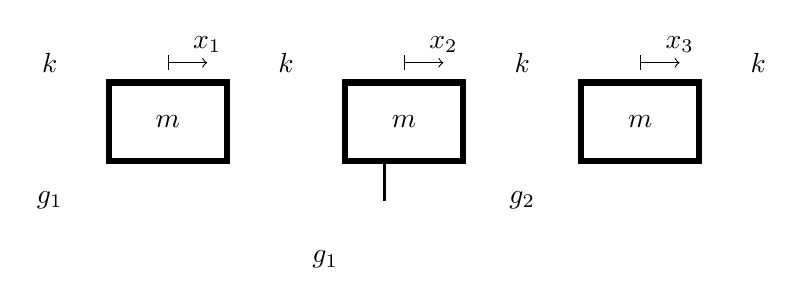
\begin{tikzpicture}
\draw[line width=.8mm](2,0)rectangle++(1.5,1);
\draw[line width=.8mm](5,0)rectangle++(1.5,1);
\draw[line width=.8mm](8,0)rectangle++(1.5,1);
\setstructmech{linewidth=.4mm}
\Spring{.5,.75}{2,.75}{1.5}
\Spring{3.5,.75}{5,.75}{1.5}
\Spring{6.5,.75}{8,.75}{1.5}
\Spring{9.5,.75}{11,.75}{1.5}
\Dashpot{6.5,.25}{8,.25}{1.5}
\Dashpot{.5,.25}{2,.25}{1.5}
\Dashpot{4,-.5}{5.5,-.5}{1.5}
\FixedSupport[-90]{.5,.5}{2}
\FixedSupport[90]{11,.5}{2}
\FixedSupport[-90]{4,-.5}
\draw[line width=.4mm](5.5,-.5)--++(0,.5);
\draw[|->](2.75,1.25)--++(.5,0)node[above]{$x_1$};
\draw[|->](5.75,1.25)--++(.5,0)node[above]{$x_2$};
\draw[|->](8.75,1.25)--++(.5,0)node[above]{$x_3$};
\node at(2.75,.5){$m$};
\node at(5.75,.5){$m$};
\node at(8.75,.5){$m$};
\node at(1.25,1.25){$k$};
\node at(4.25,1.25){$k$};
\node at(7.25,1.25){$k$};
\node at(10.25,1.25){$k$};
\node at(1.25,-.5){$g_1$};
\node at(4.75,-1.25){$g_1$};
\node at(7.25,-.5){$g_2$};
\end{tikzpicture}
\caption{three DOF system with two exponential kernels}\label{fig:three_dof}
\end{figure}
The parameters are set to $m=3$, $k=2$ and
\begin{gather}
g_1=\num{0.6}\exp\left(-t\right),\qquad
g_2=\exp\left(-5t\right).
\end{gather}
The initial conditions are $x_1\left(0\right)=1$, $x_2\left(0\right)=x_3\left(0\right)=0$, and $\dot{x}_1\left(0\right)=\dot{x}_2\left(0\right)=\dot{x}_3\left(0\right)=0$. One can compute the initial acceleration using the analytical solution such that $\ddot{x}_1\left(0\right)=-4/3$, $\ddot{x}_2\left(0\right)=2/3$ and $\ddot{x}_3\left(0\right)=0$.
The analytical solution can be obtained via modal analysis/expansion, the relevant derivations can be seen elsewhere \citep{Wagner2003}.

The displacement histories of three DoFs are depicted in \figref{fig:three}.
\begin{figure}[H]
\centering
\includegraphics{PY/three_dof}
\caption{displacement history and error analysis of three DOF system with two exponential kernels}\label{fig:three}
\end{figure}

Compared to the numerical solutions (with $\Delta{}t=\SI{0.05}{\second}$) obtained by \citet{Cortes2009}, the present algorithm yields more accurate results. Even for a large time step $\Delta{}t=\SI{0.1}{\second}$, there is no severe deviation observed, unlike some other methods \citep{Puthanpurayil2014,Liu2014} that poorly integrate the convolution term. Additional error convergence comparisons can be seen elsewhere \citep{Liu2023}. The convergence of absolute error again shows a quadratic order, implying the simple \eqsref{eq:eqv_sys} is effective.
\subsection{Three DOF System With Stiff Exponential Kernels}
The two exponential kernels in the previous example are modified to investigate whether the proposed algorithm can cope with stiff problems. The following functions are chosen.
\begin{gather}
g_1=600\exp\left(-1000t\right),\qquad
g_2=400\exp\left(-2000t\right).
\end{gather}

The corresponding displacement history and error convergence are shown in \figref{fig:three_stiff}. With a large $\mu$, the system behaves more like a viscously damped one.
\begin{figure}[H]
\centering
\includegraphics{PY/three_stiff}
\caption{displacement history and error analysis of three DOF system with stiff exponential kernels}\label{fig:three_stiff}
\end{figure}
The second-order convergence is not affected by the stiff kernel used. This is difficult to achieve with methods that explicit integrate the convolution term if the large time step is not split into smaller segments. Consider a time step of $\Delta{}t=\SI{0.01}{\second}$,
\begin{gather}
g_1\left(0\right)=600,\qquad
g_1\left(0.01\right)\approx\num{0.027},\qquad\int_{0}^{0.01}g_1~\md{t}\approx0.599973.
\end{gather}
Such a rapidly changing function within $t\in[0,0.01]$ can hardly be accurately integrated by solely using values at two ends.
\subsection{Three DOF System With Two Gaussian Kernels}
In the previous example, instead of two exponential kernels, two Gaussian kernels
\begin{gather}
g_1=1.2\sqrt{\dfrac{1}{\pi}}\exp\left(-t^2\right),\qquad
g_2=0.4\sqrt{\dfrac{5}{\pi}}\exp\left(-5t^2\right),
\end{gather}
can be used. The sum-of-exponential approximations given by the VPMR algorithm are shown in \figref{fig:vpmr}. With a tolerance around \num{e-12}, only \num{13} exponentials are required. The corresponding $m_l$ and $s_l$ parameters are given in \secref{sec:vpmr}.
\begin{figure}[H]
\centering
\includegraphics{PY/kernel}
\caption{approximations of Gaussian kernels using VPMR algorithm}\label{fig:vpmr}
\end{figure}

\begin{figure}[H]
\centering
\includegraphics{PY/three_gauss}
\caption{displacement history of three DOF system with two Gaussian kernels}\label{fig:three_gauss}
\end{figure}
For $\Delta{}t\approx\num{e-3}$, quadratic convergence implies the error is around \num{e-6}. In such a condition, the tolerance \num{e-12} used for kernel approximation is considered accurate. In practice, one can determine the tolerance based on the time step size, which can be chosen based on the properties of the dynamic system of interest, such that a proper number of exponentials would be used to balance between accuracy and efficiency. \figref{fig:three_gauss} compares the results with different time step sizes. Numerical results obtained by using other methods can be seen elsewhere \citep{Shen2021}.

For this particular example with a few DoFs and elements, the extra time required by nonviscous damping (\num{13} exponentials) is around \SI{15}{\percent} of total analysis time. Noting that the approximation of kernel is computed offline and does not change with the size of dynamic system, it can be extrapolated that for large systems, the cost of computing \eqsref{eq:composition} is not subtle.
\subsection{A Frame Structure}

\begin{figure}[H]
\centering
\includegraphics{PY/kernel2}
\caption{sigmoid kernel}\label{fig:sigmoid_kernel}
\end{figure}